\section{Baza de date}

	Tabelele din baza de date sunt denumite cu pluralul obiectului la care se referă, folosind în loc de spații sublinia „\_”.
	Puteți observa în detaliu diagrama bazei de date la figura~\ref{fig:database_diagram}

	\begin{figure}
		\centering
		\vspace*{-1.4in}
		\hspace*{-0.5in}
     		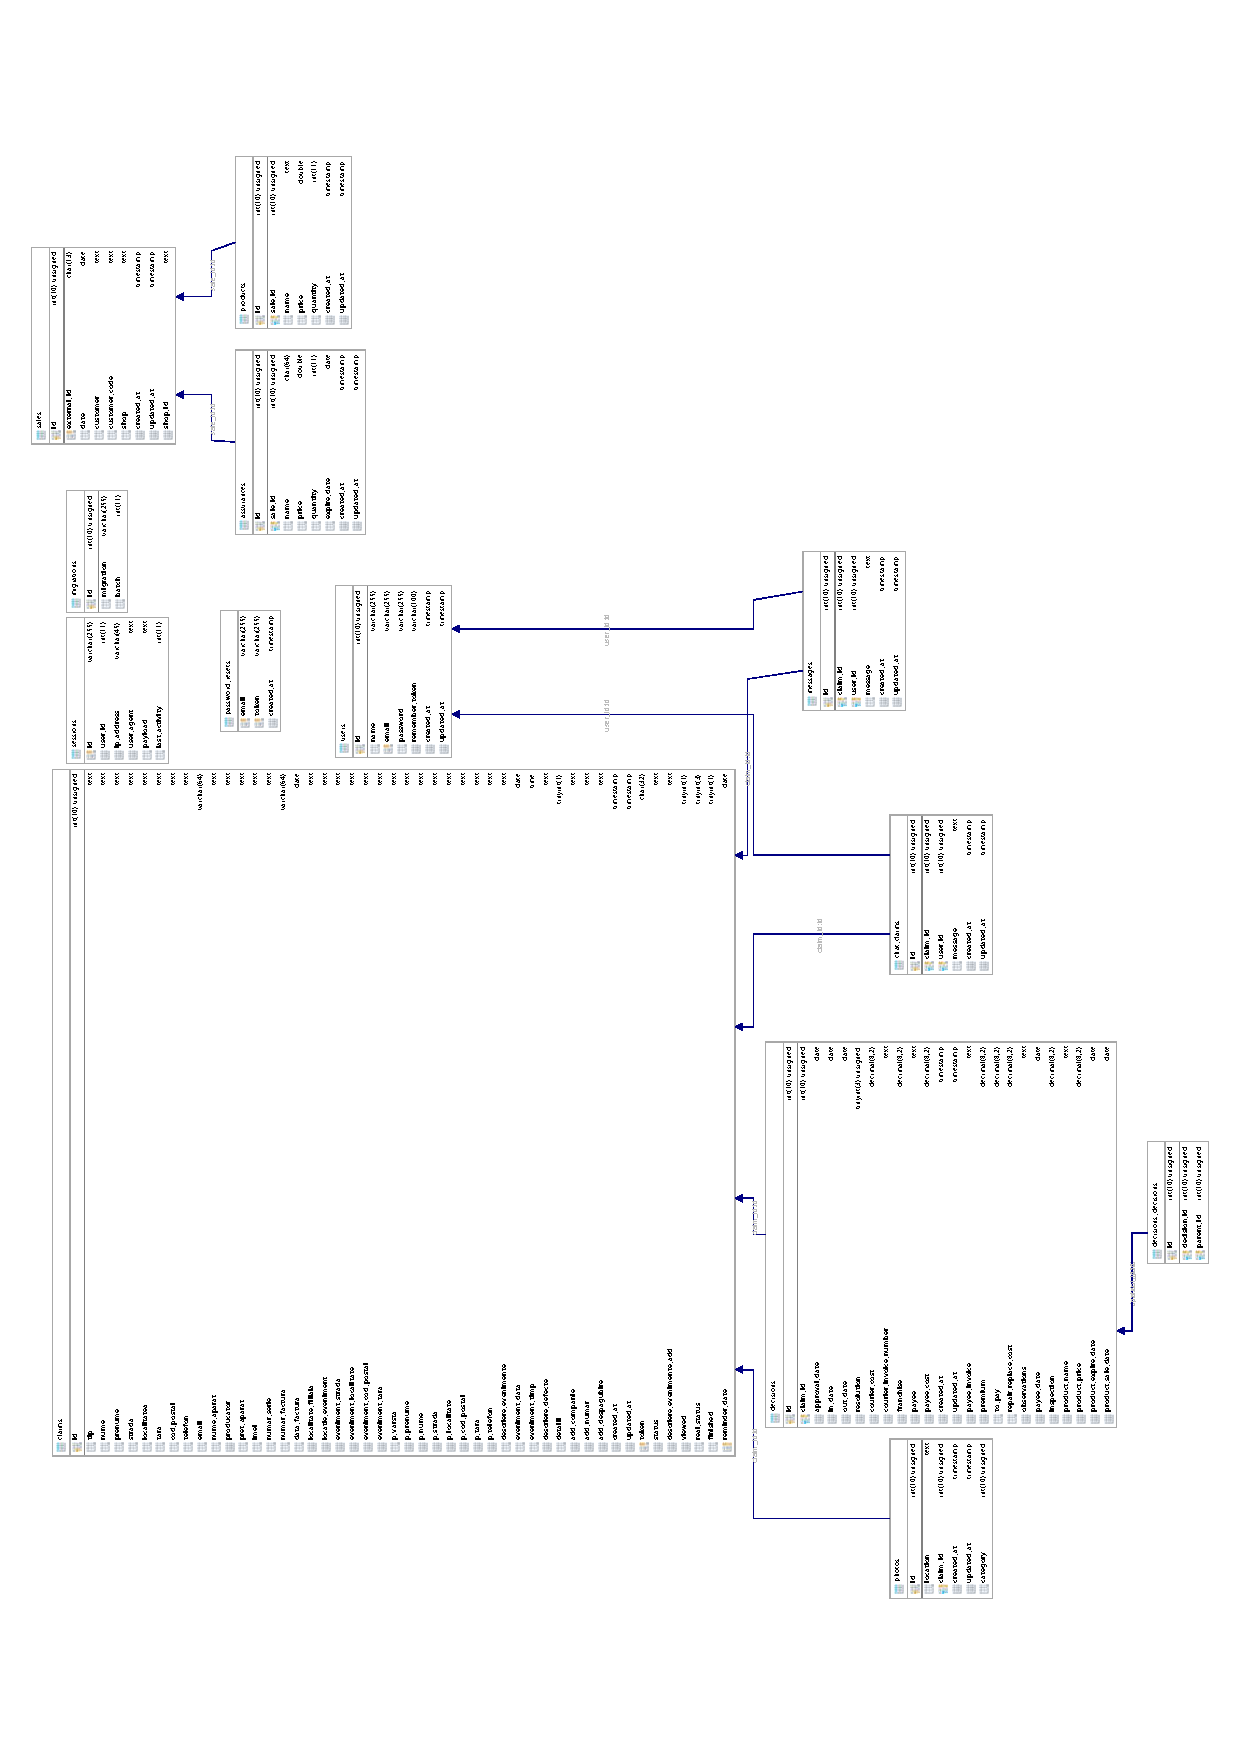
\includegraphics[width=1.1\textwidth,height=1.2\textheight,keepaspectratio]{../imagini/database_diagram.pdf}
		\caption{Diagrama bazei de date}
		\label{fig:database_diagram}
	\end{figure}


	Aceasta este salvată o dată pe săptămână și conține datele despre:
	\begin{enumerate}
		\item \verb|claims| - Cererile de despăgubire.
		\item \verb|sales| - Vânzări, cu legăturile de cheie primară (una-la-multe) la următoarele tabele:
			\begin{enumerate}
				\item \verb|products| - Produse
				\item \verb|assurances| - Asigurări
			\end{enumerate}
		\item \verb|decisions| - Decizii, cu legătura circulară folosind tabelul \\ \verb|decisions_decisions|.
		\item \verb|chat_claims| - Mesajele trimise în cadrul cererilor între utilizatorii sistemului, ce depinde de tabelul de cereri.
		\item \verb|messages| - Mesajele trimise în cadrul cererilor între client și  utilizatorii sistemului, ce depinde de tabelul de cereri.
		\item \verb|migrations| - Migrările schemei bazei de date, menținut de Laravel.
		\item \verb|users| - Utilizatorii aplicației, cu parola encriptată.
		\item \verb|photos| - Legăturile între locația pozelor și cererea, respectiv categoriilor lor, ce depinde de tabelul de cereri.
	\end{enumerate}

	\pagebreak
